\section{Creating a BT structure}
    There are several possible approaches to creating a BT structure. We will present several of these approaches and state the used one. In this section, we used the insight from \cite{BT_creation}.\\
    The first approach is creating the complete BT by hand. Meaning that humans must design every node and its position and function within the structure.\\
    The second approach is creating an initial BT and letting RL algorithms improve their functionality and optimality. There are a few options for this approach.\\
    The third possible approach is constructing the BT from previously recorded human behavior.\\
    The last possible approach lets the RL algorithm construct the BT structure from scratch.\\\\
    \bfc{Chosen approach}\\
    We have chosen the first approach, meaning we will construct the whole tree structure by hand. This was done as it is the easiest approach to this task and does not require any additional steps.\\
    Using different approaches to designing and improving the BT structure may be an interesting task for future work.\\
    We will design the BT structure in the GUI application designed alongside our chosen BT library, Groot. The application interface is shown in figure \ref{fig:groot}.
    \begin{figure}[ht]
        \centering
        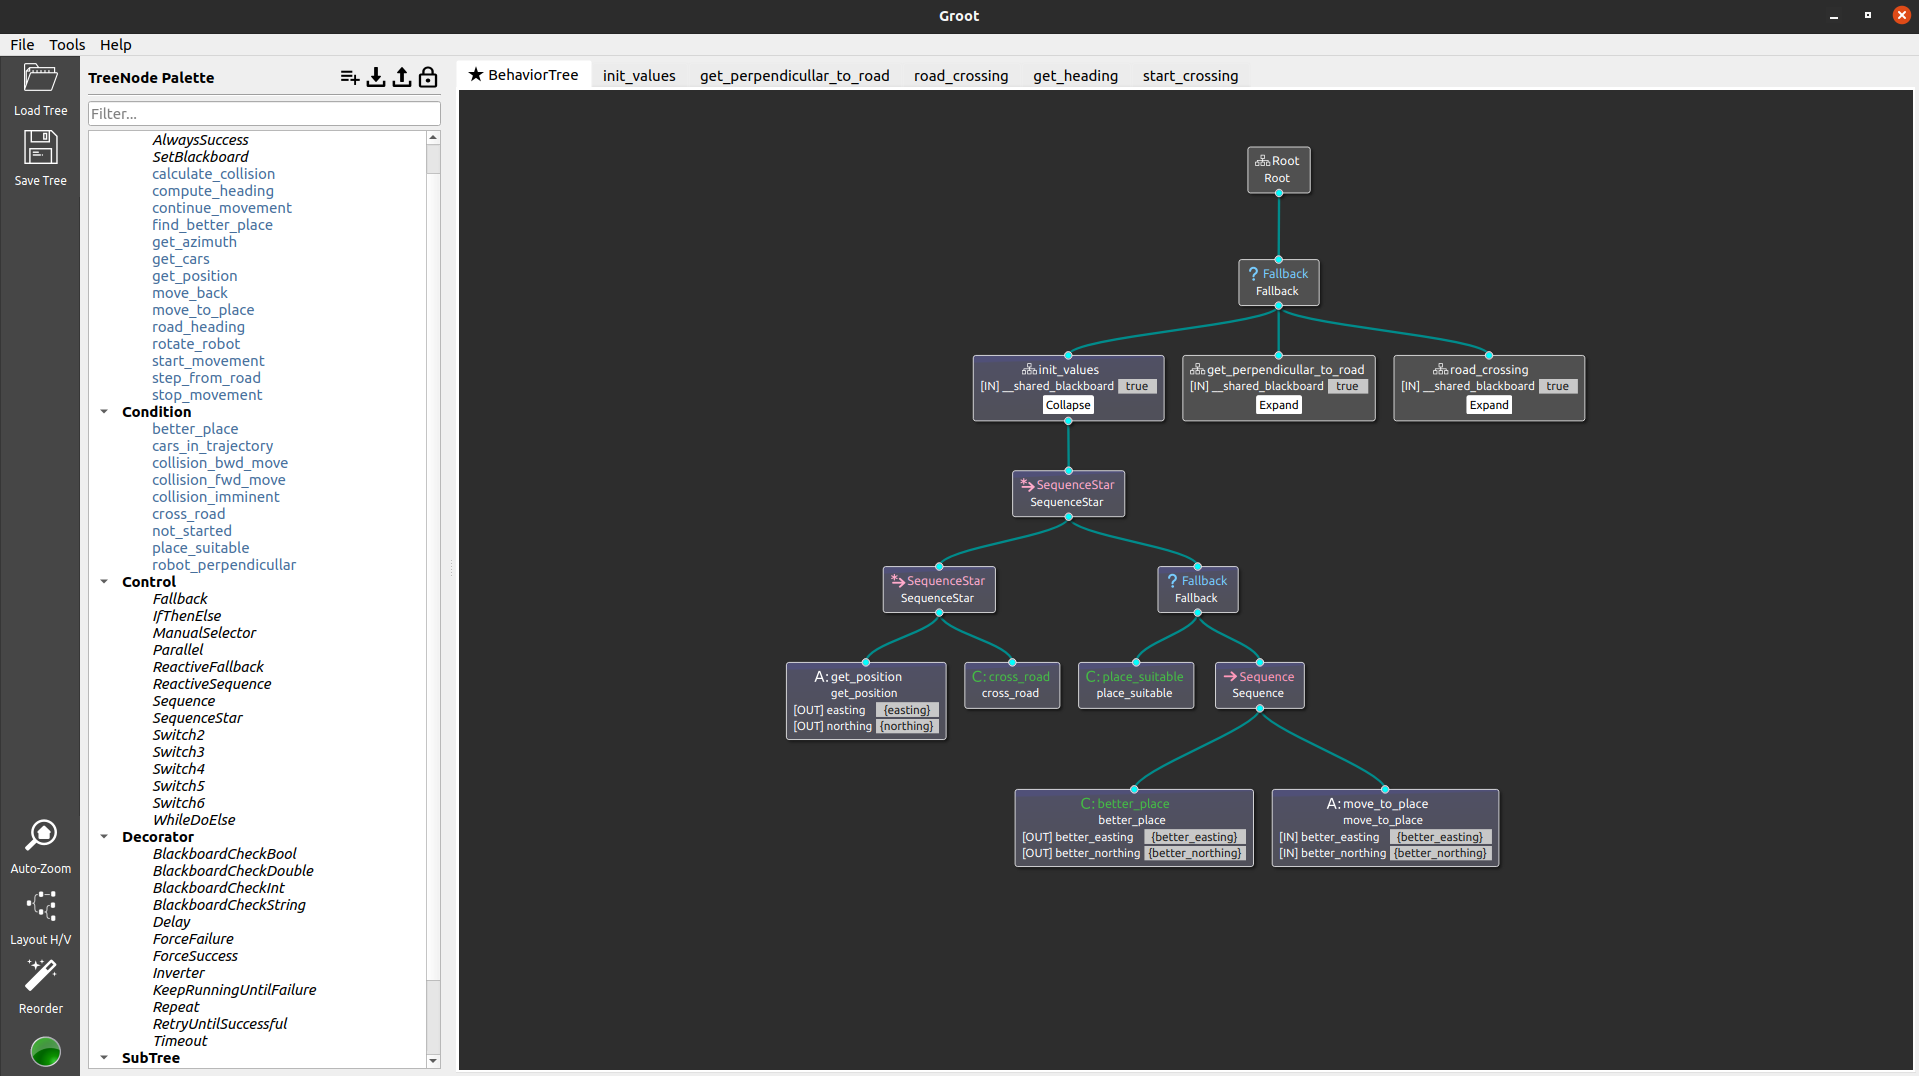
\includegraphics[width=\linewidth]{images/Groot.png}
        \caption{The Groot application interface.}
        \label{fig:groot}
    \end{figure}

\section{Structure hierarchy}
    We will divide the whole tree structure into several sub-trees to help with readability, modularity, and maintainability.\\
    The first sub-tree will help with initialization and will be responsible for determining whether the tree should be run. It is also responsible for navigating the robot to a suitable crossing place. This sub-tree will be called \texttt{Init-BT}.\\
    The second sub-tree will be responsible for positioning the robot such that it is perpendicular to the road it is trying to cross. This sub-tree will be called \texttt{Perpendicular-BT}.\\
    The third sub-tree will be responsible for the navigation of the robot during the crossing. It will check the positions and speed of incoming traffic and determine the best strategy for the crossing. This sub-tree will be called \texttt{Crossing-BT}.\\
    There are a few more sub-trees in our structure, but those are not that important to write about here. They will be presented when they are mentioned in the main sub-trees structure. Their main task is to help with the modularity and reusability of the behavior they encode.
    The main BT is shown in figure \ref{fig:main-BT}.
    \begin{figure}[ht]
        \begin{tikzpicture}[sibling distance=30mm, minimum width=1cm, minimum height=0.8cm]
            \node [draw] {$Root$}
                child {node [draw] {$\to$} edge from parent [-{Stealth[length=2.5mm]}]
                child {node [ellipse, draw] {StartAlgorithm}}
                child {node [draw] {$\to^{*}$}
                child {node [diamond, draw, aspect=2.3, xshift=0-1cm, yshift=0-0.5cm] {Init-BT}}
                child {node [diamond, draw, aspect=2.3, yshift=0-0.5cm] {Perpendicular-BT}}
                child {node [diamond, draw, aspect=2.3, xshift=1.5cm, yshift=0-0.5cm] {Crossing-BT}}}};
        \end{tikzpicture}
        \caption{Main BT structure.}
        \label{fig:main-BT}
    \end{figure}

\section{Init-BT}
    As mentioned earlier, this BT is responsible for determining if we should start the crossing and for navigating the robot to the optimal location. This tree will be executed only once for each crossing. We accomplish this with a \texttt{SequenceStar} node as the first node after \texttt{Root}. The \texttt{Init-BT} structure is shown in figure \ref{fig:Init-BT}.
    \begin{figure}[H]
        \begin{tikzpicture}[sibling distance=28mm, minimum width=1cm, minimum height=0.8cm]
            \node [draw] {$Root$}
                child {node [draw] {$\to$} edge from parent [-{Stealth[length=2.5mm]}]
                child {node [draw] {$\to^{*}$}
                child {node [draw] {GetPosition}}
                child {node [ellipse, draw] {CrossRoad}}}
                child {node [draw, xshift=1cm] {$\checkmark$}
                child {node [draw] {$\circ(10)$}
                child {node [draw] {?}
                child {node [ellipse, draw] {PlaceSuitable}}
                child {node [draw] {$\to$}
                child {node [ellipse, draw, xshift=0-0.1cm] {BetterPlace}}
                child {node [draw, xshift=0.1cm] {MoveToPlace}}}
                child {node [draw] {GetBetterPlace}}}}}};
        \end{tikzpicture}
        \caption{The Init-BT structure.}
        \label{fig:Init-BT}
    \end{figure}
    \noindent The flow for the algorithm is the following. First, we need to check if the algorithm should be even started -- to avoid collision between two nodes trying to control the robot. This we achieve with a \texttt{StartAlgorithm} node. The next node after this one is \texttt{GetPosition} followed by a condition \texttt{CrossRoad}. They are connected in one \texttt{SequenceStar} control node. The whole point of this sub-structure is to determine the proximity of the robot to the road. If the robot is too far away from the road, the algorithm should not progress. This will help combat the possibility of trying to cross the wrong road, should it happen that two roads are close by.\\
    The next major sub-structure is behind a \texttt{Fallback} node. The idea behind this one is to place the robot in an ideal position for crossing. This action should have been done before the mission, and the robot should have been sent to the optimal location by a path-planning node. However, if that was not performed, the \texttt{PlaceSuitable} condition node will check if the place is suitable. If not, the \texttt{BetterPlace} condition node will show if a better location was found. An action node \texttt{MoveToPlace} will steer the robot to a better location if it has been found. Lastly, the action node \texttt{GetBetterPlace} will try to find a better place. We will not perform the sub-tree again if a better place cannot be located. Instead, we will move on to the following sub-tree.

\section{Perpendicular-BT}
    This sub-tree is responsible for positioning the robot for crossing in the most optimal way. We have determined that to be the one in which the robot will cross the road the fastest. As such, the position of the robot should be perpendicular to the road it is going to cross. Figure \ref{fig:Perpendicular-BT} shows the BT structure for achieving so.
    \begin{figure}[H]
        \begin{tikzpicture}[sibling distance=28mm, minimum width=1cm, minimum height=0.8cm]
            \node [draw] {$Root$}
                child {node [draw] {$\to^{*}$} edge from parent [-{Stealth[length=2.5mm]}]
                child {node [draw] {$\to^{*}$}
                child {node [draw] {$\circ(10)$}
                child {node [draw] {GetAzimuth}}}
                child {node [draw, xshift=0-0.7cm] {$\circ(10)$}
                child {node [draw] {$\to$}
                child {node [draw, xshift=0.65cm] {GetPosition}}
                child {node [draw, xshift=0.35cm] {RoadHeading}}
                child {node [draw, xshift=0.5cm] {ComputeHeading}}}}}
                child {node [draw, xshift=3cm] {$\circ(10)$}
                child {node [draw] {$\to$}
                child {node [draw] {GetAzimuth}}
                child {node [draw] {?}
                child {node [ellipse, draw, xshift=0-0.5cm, yshift=0-1.5cm] {RobotPerpendicular}}
                child {node [draw] {$\times$}
                child {node [draw] {?}
                child {node [draw, xshift=0-1.2cm] {RotateRobot}}
                child {node [draw, xshift=0-1.2cm] {StepFromRoad}}}}}}}};
        \end{tikzpicture}
        \caption{The Perpendicular-BT structure.}
        \label{fig:Perpendicular-BT}
    \end{figure}
    \noindent This tree is also only needed once in each run of the crossing algorithm therefore, we start with a \texttt{SequenceStar} node after \texttt{Root}.\\
    The first significant sub-structures task is determining the azimuth for the robot to be perpendicular to the road. This also does not need to be repeated for a single road, so we start with a \texttt{SequenceStar} control node, next, we have a \texttt{Repeat} node. The action to be repeated is the obtaining of the robot's azimuth. The following steps are also behind a \texttt{Repeat} control node. This part of the algorithm calculates the azimuth the robot should have to be perpendicular. Firstly we need to obtain the robot's position -- \texttt{GetPosition} action node. Next, we need to determine the road heading closest to the robot. For this purpose, we have the action node \texttt{RoadHeading}. Finally, we calculate the proper azimuth for the robot with the action node \texttt{ComputeHeading}. This concludes the left branch of our Perpendicular-BT.\\
    The right branch starts with a \texttt{Repeat} node, followed by a \texttt{Sequence} node. The idea behind this branch is to utilize the azimuth value computed in the left branch and orient the robot accordingly. Firstly we need to obtain the robot's azimuth with the \texttt{GetAzimuth} action node. While this might seem redundant, we have just got the azimuth for calculation, it is vital to update the current azimuth as the value of obtained azimuth is only valid in the first run of the second branch. After receiving the current azimuth, we follow with a \texttt{Fallback} node and its first child, a condition node \texttt{RobotPerpendicular}. This node tells us if the robot has achieved the optimal azimuth we calculated earlier. If it has not, we continue, thanks to the \texttt{Fallback} node to the last part of this sub-tree. We want this part to always return \texttt{FAILURE}. This is necessary because we check the correct position before the movement. The last part is responsible for the movement of the robot. Firstly we try to rotate the robot with \texttt{RotateRobot} action node. If the rotation was unsuccessful, we tried to move the robot away from the road with \texttt{StepFromRoad}. This is implemented as the robot rotation could have brought the robot onto the road, which is forbidden.\\
    While we could unite the first two \texttt{Repeat} nodes, maybe even all three, we chose not to do so. The reason for not merging the nodes is to allow each algorithm part to fail independently. The number of repetitions for each node was set to 10, which we determined to be the optimal value.
